\documentclass[a5paper,11pt]{article}
\usepackage[utf8]{inputenc}
\usepackage{graphicx}
\usepackage[svgnames]{xcolor}
\usepackage{minted}
\usepackage[ampersand]{easylist}
\usepackage{fancyvrb}
\usepackage[top=1in]{geometry}
\usepackage{hyperref}
\usepackage{framed}
\usepackage{titling}


\usepackage{transparent}
\usepackage{eso-pic}
\usepackage{blindtext}
\usepackage{tikz}


\makeatletter
\renewcommand{\@seccntformat}[1]{}
\makeatother

\setlength{\parskip}{1em}
\setlength{\parindent}{0pt}

\title{}
\date{}
\begin{document}

\newcommand{\BackgroundPic}[1]{%
\put(0,0){%
\parbox[b][\paperheight]{\paperwidth}{%
\vfill
\centering
{\transparent{0.6} \includegraphics[width=\paperwidth,height=\paperheight]{#1}}%
\vfill
}}}

\newcommand{\TitlePic}[1]{%
\put(0,0){%
\parbox[b][\paperheight]{\paperwidth}{%
\vfill
\centering
{\transparent{0.9} \includegraphics[width=\paperwidth,height=\paperheight]{#1}}%
\vfill
}}}


\begingroup
\let\cleardoublepage\clearpage

\AddToShipoutPictureBG*{\TitlePic{TwineTitle}}
\begin{titlingpage}
  \maketitle
\end{titlingpage}
\endgroup
 
\newpage

\tableofcontents

\newpage 
\section{Introduction to Twine}
Twine is a system for making \emph{interactive stories}, that is stories where the reader has actual choices, decisions, and ways to interact with the story. Think something like a \emph{Choose Your Own Adventure} book or more modern stories like \emph{Life is Strange}.

The thing that makes Twine so great is that you can easily get started writing a story with just a handful of concepts and basically no code at all.

Let's put our money where my mouth is and start making a story!
\newpage
\section{Making your first story}
\subsection{First steps}
To get started with Twine

\begin{itemize}
 \item Go to the main Twine website \url{http://twinery.org}. 
 \item Click on the link that says \verb"use it online"
 \item Click on the link that says \verb"skip"
 \item Click on the \verb"+Story" link
 \item Give your story a name
\end{itemize}

That should bring you to a screen that looks like

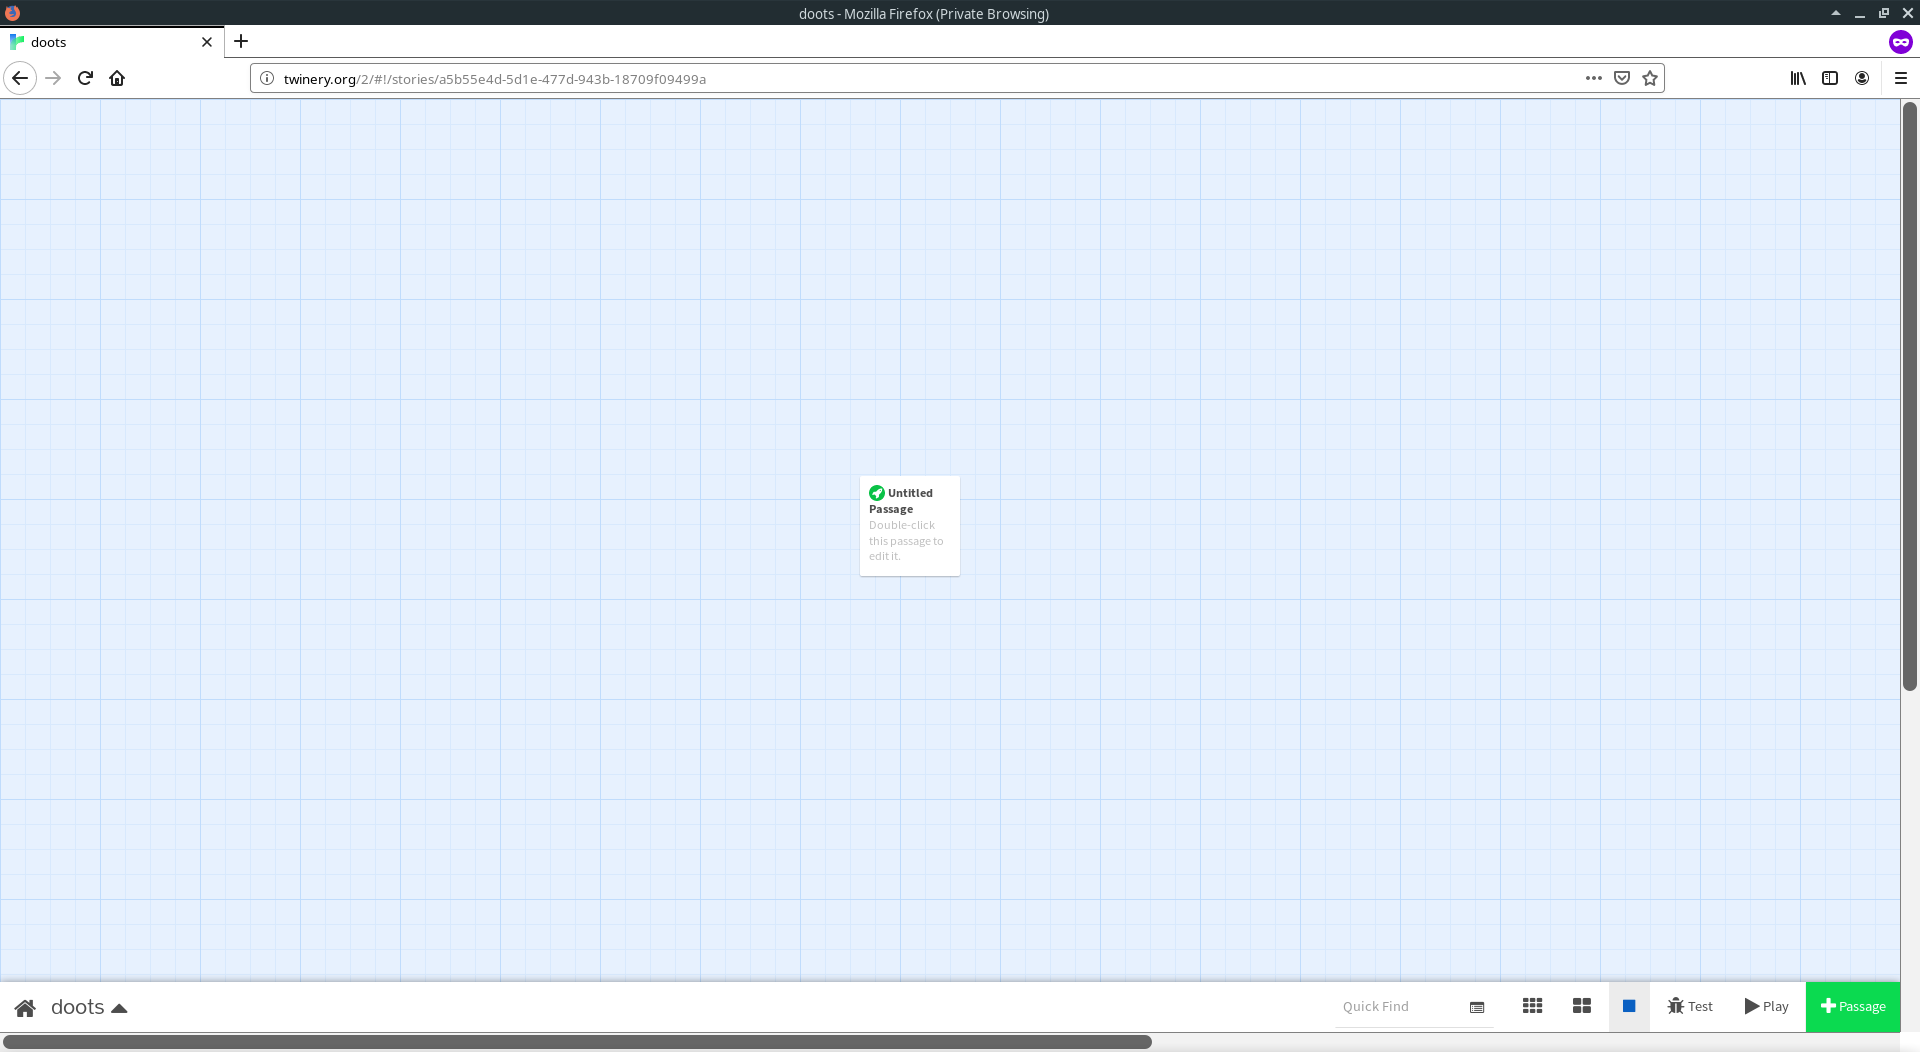
\includegraphics[width=1.1\linewidth]{TwineHome}

From here, you can double click on the white square in the middle of the screen and get started writing a scene. 
\subsection{Describing a scene}
Assuming you double clicked on the white square that said ``Untitled passage'' you should have a pop-up that looks like

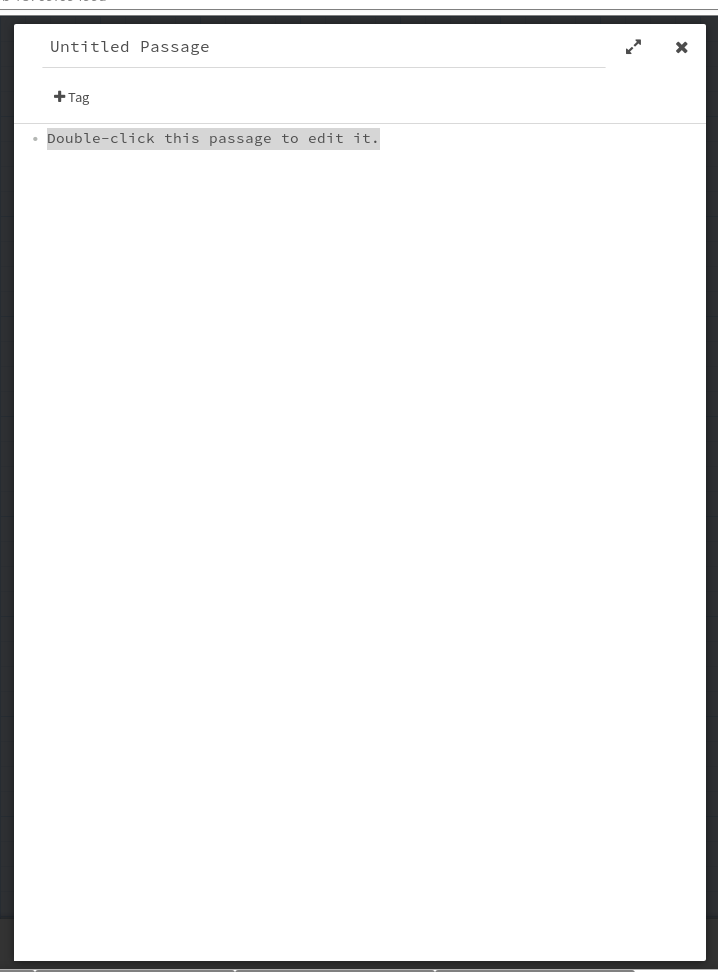
\includegraphics[width=0.9\linewidth]{EditPassage}

This is a \emph{passage}, where we write the text of our stories.

\begin{framed}
  You should now try writing some text in this window.

  Describe a place, real or imaginary, and include details about what's in the place. Don't think of this part as coding, just write it like you're writing a story. When you're done, give the scene a title by replacing the text that says ``Untitled passage''
\end{framed}

Once you've written down a scene, click out of the pop-up window and then hit the \verb"Play" button in the lower right-hand corner of the screen.

You should see your story so far displayed on the screen! Thankfully, we can do more than just write a single scene in Twine. Our next task is to add \emph{choices} to our story.
\subsection{Making choices}
Our interactive story wouldn't be very interactive if we couldn't make choices!

In Twine, our choices are called \emph{links}. Links connect different passages together. As an example, if we have a passage with the text
\begin{verbatim}
Your eyes fly open to see that you're 
no longer in your bedroom but, in fact, 
in a room with two doors: 
 [[a red door]] and [[a blue door]].
\end{verbatim}
this passage has two links with the text \texttt{a red door} and \texttt{a blue door} which in turn create two new passages called \texttt{a red door} and \texttt{a blue door} respectively.

You don't always want the text of the link to be the same as the name of the passage it's linking to. For example, imagine that when a player dies you want them to go back to the beginning passage, which is titled ``The start''. But you don't want the player to click on ``The start'' to restart the game, you want the player the player to click on a link that says ``You died, dingus!'' in order to go to ``The start''. To do that you want to write the link as
\begin{verbatim}
[[You died, dingus!->The start]]
\end{verbatim}

\textbf{Caution: you need to make sure the name of the passage to the right of the arrow symbol is exactly the name of the passage: upper and lower case all have to match as well as the number of spaces.}

\begin{framed}
  Take the scene you started with and add three choices as links.

  One link should be a new place to go. Another link should be a thing you can \emph{do} in the room like find a key or pick your nose. The last link should be a choice that \emph{looks} like it would take you somewhere but it takes you back to the passage you've already made. 
\end{framed}

When you're done you should be able to run your story and click on the links. If you followed the suggestion for links above two of them are going to lead to passages where the only text is

\texttt{Double click this passage to edit it}.

Now with just these few skills you can keep working on passage after passage, adding links as you go, until you make an entire story!

\section{Saving and restoring your work}
When you want to save your story there's a few things to consider:
\begin{itemize}
  \item If you're on a computer you own you can just close your browser when you're done working on your story. Everything has been automatically saved \textit{as long as you don't clear your browser data.}
  \item If you're on a computer you \emph{don't} own then you need to re-save your work every time you're done by clicking on the black triangle in the lower left-hand corner of the screen and choosing the option that says ``Publish to File''. You'll want to put this \verb".html" file on a thumb drive, move it to online storage like Google Drive, or email it to yourself.
  \end{itemize}

  \begin{figure}[h]
    \caption{The menu to save your story}
    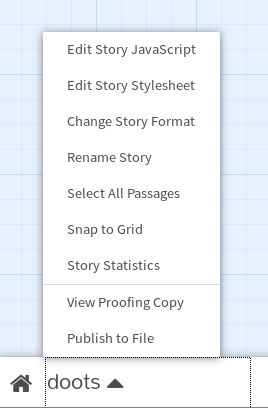
\includegraphics[width=0.6\linewidth]{SavingTwine}
    \centering
  \end{figure}
  
  If you \emph{manually} saved your Twine story, you can restore it later by going to the main Twine menu and choosing ``Import From File'' instead of adding a new story. Otherwise, you can just click on the story from the left-hand menu.

\clearpage

  \section{Introduction to Harlowe}
You can do a lot more in Twine than just make links and passages! To do that, though, you're going to need to start writing code!

In Twine, this means learning how to program in a special programming language called \emph{Harlowe}. Harlowe commands generally look something like
\begin{verbatim}
(command: arg1, arg2, arg3)[text that the command modifies]
\end{verbatim}

For example,
\begin{verbatim}
(set: $dogsFound to 0)
\end{verbatim}
puts the value \verb"0" inside a variable named \verb"$dogsFound".

The code
\begin{verbatim}
(if: $dogsFound is 3)[You found all the dogs!]
(else:)[Why are you talking to me go find the dogs!?]
\end{verbatim}
makes the passage display different text depending on how many dogs have been found in the game.

If three dogs have been found and you visit this passage, you'll see "You found all the dogs!". Otherwise, you'll see "Why are you talking to me go find the dogs!?".

We'll explain exactly how the code above works in more detail later in the guide! Be warned, though, that the following tutorial/reference is still only a small fraction of what you can do in Harlowe.

The complete documentation for Harlowe is available on \url{http://twine2.neocities.org}. There you can look up any possible Twine command and how it works with examples.
\subsection{Making and using variables}
In essentially all programming languages, there is a way to store data in ``named containers'' called \emph{variables}. Harlowe is no exception!
In Harlowe you can make variables by ``setting'' them. which gives them a value that you can use later. You can get the value stored inside the variable by just using the variable's name in the text.

\textbf{Caution: all variable names in Harlowe must start with a \$}.

Here's an example:
\begin{verbatim}
(set: $weightOfAFatDog to 20)

Oh boy, that dog is so fat. 
I bet it weighs $weightOfAFatDog pounds, more or less!
\end{verbatim}

When Twine renders this text in a passage it will replace the variable with its value and produce the text ``Oh boy, that dog is so fat. I bet it weighs 20 pounds, more or less!''.

Once you set a variable in a passage, it \emph{stays} set in future passages. 

\subsection{Choices and if-statements}
What if you want different things to happen in your story depending on what events \emph{already} happened? In programming, this is generally done with something called an if-statement or an if-then-statement. It allows you to make decisions of the form ``if it's raining, then put up your hood'' or ``if you have change, go play pinball after school''.

To do that in Harlowe, you can say
\begin{verbatim}
(if: $hp < 3)[The healing potion 
restores your health. (set: $hp to 3)]
\end{verbatim}
This code checks to see if a variable called \verb"$hp" is less than 3 and, if it is, then display the text that's \emph{inside the single square brackets}. Note that we can put more Harlowe code between the square brackets that come after the \verb"if". The code inside the square brackets will only run if the condition in the \verb"if" is true. 

\textbf{Caution: be sure to not put a space between the} \verb")" \textbf{and the} \verb"[" \textbf{or else Harlowe will get confused}

What if you want something that logically looks more like ``if it's raining, then put up your hood, otherwise put on sunscreen''. To do that in Twine, you need to use a thing called \verb"(else:)" like in the following example.

\begin{verbatim}
(if: $relationship > 50)["Omigosh!" they exclaim. 
"I will go to Canada with you!"]
(else:)["Umm we've only had one date, 
 you know that right? This is weird."]
\end{verbatim}

\subsubsection{Making a link conditional}
So sometimes you might want to make whether a link appears conditional. Imagine a story where you only want the player to ask another character about something, like flying pink frogs, \textit{after} they've learned that flying pink frogs exist.

To do something like this you'll put the link \textbf{inside} the if-statement, but there's a tricky bit with the formatting: you need to put spaces around the link or else Harlowe gets confused about what the link is.

Thus you need to format your link like

\begin{verbatim}
(if: $knowsAboutPinkFrogs)[ 
[[Ask her about the weird frogs you saw]] ]
\end{verbatim}
and not like

\verb"[[[Ask her about the weird frogs you saw]]]"

\subsubsection{Conditionally returning values}
Sometimes you'll want to just do \emph{one thing} with your choice, and that's choose \emph{a} value based on which of a set of possible things are true. For example, let's say you have a roleplaying game with character classes and you want to set a starting weapon based on the class the player selected. For example, if you put the following code in a passage and play it you should see the text ``As a clown, you ready your shoes''.

\begin{verbatim}
(set: $class to "clown")

(set: $weapon to (cond: $class is "bard", "harp", 
 $class is "knight", "sword", 
 $class is "clown", "shoes"))
 
As a $class, you ready your $weapon
\end{verbatim}

\subsection{Changing colors and fonts}
If you're writing a big story with lots of text, you might want to change up the font, text color, or even apply some special effects to catch the Player's eye.  The good news is that in Twine those things are pretty straightforward!

You can change the color of text with the \verb"color" command like in the following example
\begin{verbatim}
(color: cyan)[This text should be blue!]
\end{verbatim}


\includegraphics[width=0.7\linewidth]{cyantext}


Harlowe has a number of colors pre-defined like \verb"red", \verb"white", or \verb"yellow". Can you use more colors than that? Absolutely! If you look up the hex code of a color with a site like \url{https://htmlcolorcodes.com/color-picker/} then you can just enter the hex code into the \verb"color" command like

\begin{verbatim}
(color: "#1abc9c")[This text should be teal]
\end{verbatim}


\includegraphics[width=0.7\linewidth]{tealtext}

Beyond changing the color, you can also change the font of your text! Now if you want to change the font to something that's pretty standard across the web then all you need to do is type something like

\begin{verbatim}
(font: "Courier New")[And the text is going
to look like a typewriter]
\end{verbatim}

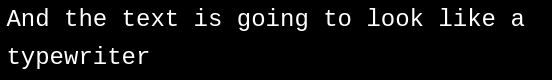
\includegraphics[width=0.7\linewidth]{couriertext}


Fonts you can easily use include stuff like
\begin{itemize}
\item Courier New
\item Arial
  \item Times New Roman
\end{itemize}

But, in general, if you want some super cool looking font you're going to have to do some setup work to make sure that the player's browser has the right fonts loaded.

I think the easiest way to do this is to use Google fonts

\url{https://fonts.google.com}

From here you can click on the little plus sign of any font that you think looks cool. Once you have you should see at the bottom of your browser a little note about ``\# Family Selected''. If you click on that you should see some text explaining how to use the font. So I selected the Lobster font, which means that Google tells me I need to load the font like
\begin{verbatim}
<link href="https://fonts.googleapis.com/css?family=Lobster" 
 rel="stylesheet">
\end{verbatim}

Now! You need to make a new passage, it's actual name doesn't matter, but you're going to click on the thing that says tag and give it a tag of \texttt{header}. When a passage has the header tag it means that it'll silently load at the beginning of every passage before the ``real'' passage you're on. Go ahead and copy and paste the link you got from Google into your header passage, then in any passage you should be able to use the font like normal.

In our case we type
\begin{verbatim}
(font: "Lobster")[a bunch of stuff 
and it should look super different]
\end{verbatim}
and it'll look, well, super different!


\includegraphics[width=0.9\linewidth]{LobsterScreenshot}

The last thing is that you can do some pretty weird things with the Harlowe command \verb"text-style". For example, the following code will make the text on the screen shudder continuously!
\begin{verbatim}
(text-style: "shudder")[OMG I'm shaking!]
\end{verbatim}
\subsection{Hooks: making links that do all sorts of things}
One thing you might be wondering is how we can make ``links'' that do more interesting things when you click on them.

There's a number of commands that can help out with that, but we'll need to talk more about hooks. We've been using hooks for awhile now. A hook is technically just [some text inside of square brackets]. In the last tutorial we were styling them, but we can do other things with them too.

We can actually give names to hooks that we can reference later in the same passage. Like the following example
\begin{verbatim}
[Something can happen up here]<tada|

(click: ?tada)[and then affect things down here]
\end{verbatim}
What this code will do is make ``Something can happen up here'' a clickable link that will make the text ``and then affect things down here'' appear below where you actually put the \verb|click| command.

So the part \verb"<tada|" is the name we gave the hook
\texttt{[something can happen up here]}. If you looked at the first tutorial and saw the way we used variables started with a \$, similarly the names for hooks start with a ? whenever you want to use them.

In this case, we just used the click command to make somthing happen when ?tada was clicked on. Here it was just to have text appear but there's a ton of things that you can do with named hooks and the documentation we linked to in Welcome to Twine! explains all the different things you can do with them and the kinds of commands you can run by interacting with text.

There's also several special hooks like \verb"?passage", \verb"?page", and \verb"?sidebar" that you can also reference to do something like making a thing happen whenever you click on a location. In a couple of sections we'll given an example of using the \verb"?passage" hook as well as a new command called \texttt{enchant}.

\subsection{Including images}
In order to break up the text of your game and keep it visually interesting, you might want to include images.

The easiest way to do this, I think, is by including \textsc{html} into your story.

If you don't know what \textsc{html} is, it's the underlying language that tells your web browser what exactly goes into a web page.

\textsc{html} is its own big topic too large to cover here, but fortunately all you need is the <img> tag. The way you use it is something like

\verb|<img src="http://bit.ly/2h9gSHn">|

which will look like

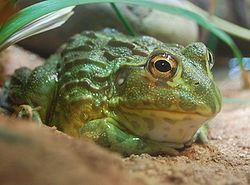
\includegraphics{froggy}

One caveat to note: you need the link to the image and not just the search result page. Make sure your URL ends in something like \verb".png" or \verb".jpg" or some other image format.

Also animated gifs do work in Twine!
\subsection{Changing the background of your passages}
Okay so you probably want to mess around with how your background looks and do things like include background images.

You can do that without too much trouble by using built in commands. So, for example, we can set a background image like
\begin{verbatim}
(enchant: ?passage, 
(background: "https://bit.ly/2GaAvbl"))
\end{verbatim}

and it will make the linked image a background in the passage, filling in the area that has text and code in it.

How did this work? Well there's a few pieces here.

First, there's the enchant command that we're using to enchant a hook rather than just a particular word. The second part is that we're using a very special hook called \verb"?passage" that refers to the entirety of the passage. There's other special hooks that Twine gives us to modify the way the entire page looks, the way the sidebar looks, and the way links look.

So if we type something like
\begin{verbatim}
(enchant: ?page, (background: red))
\end{verbatim}
we'll make the entire page red.

If you know a little \textsc{css}, Cascading Style Sheets, then you can do even more neat stuff. \textsc{css} is the tool built into every browser to that allows you web designers to customize how their pages look! You can use the \verb|css| command to create custom changers with \textsc{css} code. You don't have to do this and you're not really missing out if you don't know \textsc{css}, but if it's something you've already learned there's a lot of fun things you can change about how your game looks. 
\subsection{Enchants and changers}
You can use the enchant command with a number of other ``changers'', which is what things like \verb|background| or \verb|color| are called in the Twine documentation. One neat thing you can do with changers is \emph{store them in variables} and then use them over and over again.

The following code defines a changer that both makes the background of the text green and applies a mirror effect. Try it for yourself and see!
\begin{verbatim}
(set: $weirdChanger to 
 (background: green) + (text-style: "mirror"))
$weirdChanger[This is a secret weirdo message]
\end{verbatim}

You'll notice that to combine changers we \emph{added} them together. The enchant command has a few other interesting uses. For example, it can be used to change \emph{every instance of a word}. If we assume the same \verb|$weirdChanger| as above then
\begin{verbatim}
(enchant: "heck", $weirdChanger)
\end{verbatim}
will apply \verb|$weirdChanger| to every instance of ``heck'' in the passage. 

\subsection{Adding music}
Whether it's easy to include music in your Twine story is highly dependent on how you're distributing your story, what kind of computer you're using, how you're planning to share your story.

\subsubsection{I have the music files and a place to put them}
If you have access to some web-hosting space, then you can include the \textsc{html} code for an audio file:

You need to type
\begin{verbatim}
<audio autoplay>
<source src="awesometune.mp3" type="audio/mpeg">
</audio>
\end{verbatim}

to load the file if you've downloaded it \emph{and} have it in the same folder as your Twine story is stored.

\subsubsection{I don't have the music files or someone else is hosting the story}
What if you're hosting it somewhere free like \url{philome.la}? Or maybe the song you want is from YouTube and you want to link to a particular video? In that case, the easiest thing to do is just link to the video using hooks like we showed up above. It'll probably need to look something like
\begin{verbatim}
[Click here to play the song!]<rick|

(click: ?rick)[(
open-url: "https://www.youtube.com/watch?v=dQw4w9WgXcQ")]
\end{verbatim}

\subsection{Making a passage respond to time}
So another cool thing you can do in Twine is have your passages run code that continuously updates over time. This allows you to do things like give timed choices or force delays before new details are revealed.

The key is the live macro. You can use live to write code that will re-run over and over again as long as the player is on the passage.

So, for example, if you typed
\begin{verbatim}
(live: 1s)[
(set: $someVariable to $someVariable + 1)
$someVariable)]
\end{verbatim}
You'd see a number that keeps changing roughly once a second.

You can use this to do all sorts of cute things, like the following code that will display something only after roughly fifteen seconds. Just wait a bit for it!
\begin{verbatim}
(live: 1s)[
(set: $ourTimer to $ourTimer + 1)
(if: $ourTimer > 15)[
This message should only appear after fifteen seconds]]
\end{verbatim}
\subsection{Controlling spacing}
As you include code into your story you might notice that there's times where the spacing gets \emph{weird}. For example, if I do something like

\begin{verbatim}
You just beat the boss!
(set: $bossDead to true)
(set: $hp to 3)
(set: $hasKitchenSink to true)
And picked up the kitchen sink!
\end{verbatim}

You'll see a big gap between ``You just beat the boss!'' and ``And picked up the kitchen sink!''. That's not good! Twine doesn't skip over lines of code, since they \emph{could} potentially output text. Thankfully, there's an easy way to say to Twine ``hey, collapse all the space where there isn't literally text'' and that's the curly braces: \{ \}.

So in order to properly format our example we need to instead say
\begin{verbatim}
You just beat the boss!{
(set: $bossDead to true)
(set: $hp to 3)
(set: $hasKitchenSink to true)}
And picked up the kitchen sink!
\end{verbatim}

\subsection{Randomness}
There are a couple of ways to include randomness in your Twine game. First, if you just want to choose one of several pieces of data---like random adjectives or names---you can use the \verb|(either:)| command like in the following example
\begin{verbatim}
I can't believe you don't remember me!? 
I'm (either: "Tom","Dick","Harry")!
\end{verbatim}

The other way to add randomness is by choosing a random number! This is particularly nice for combining with the \verb|if| command.

\begin{verbatim}
(if: (random: 1,10) > 3)[
You'll only see this text 30%
of the time]
(else:)[This is going to show
up most of the time!]
\end{verbatim}

\subsection{Arrays}
We've seen that you can store all sorts of data in variables, which is great but what if you don't know how many pieces of data you need to store? What if you want to keep track of an inventory for your character or the people you've talked to etc.?

That's where you need a special kind of data to put inside your variables: arrays.

An array is basically a \emph{list} of things. You can make an array with the \verb|(a:)| command, like in the following example that uses an array with the either command. The \verb|...| you see is a way of inserting all the elements of an array into a command that's expecting a comma-separated list.

\begin{verbatim}
(set: $kindsOfWeather to 
 (a: "rainy","sunny","snowy"))
It looks (either: ...$kindsOfWeather) out
\end{verbatim}

There's also a very special array that makes a lot of advanced Harlowe coding easier: \verb|(history:)|. It contains a list of every passage you've been too in chronological order. This lets us do cool things like check to see if we've been in a passage before!

\begin{verbatim}
(if: (history:) contains (passage:)'s name)[
You've been here before]
\end{verbatim}

You can grab items out of a list like \verb|$kindsOfWeather's 1st| or \verb|(history:)'s last|. You can also check how many things are in an array like \verb|$inventory's length|. You can add things to an array with addition: \verb|(a: 1,2,3) + (a: 4,5,6)| will produce an array \verb|(a: 1,2,3,4,5,6)|

Now, there's also a \verb"-" operator as well. It doesn't work the way you might expect, though! You might think that something like \verb|(a: 1,2,1,3,1) - (a: 1)| would give you an array of \verb|(a: 2,1,3,1)| or \textit{maybe} \verb|(a: 1,2,1,3)|. What it \textbf{actually} computes is \verb|(a: 2,3)|. Subtracting one array from another means removing \textit{all} of the items in the first array that are in the second array.

\subsection{Special tags: header, footer, and startup}
You may have noticed that you can make passages with the \verb"+Passage" button. You may have even noticed that there's the ability to add tags to a passage. There are three special tags that change how your story flows: header, footer, and startup.

They all work pretty similarly! If you give a passage the header tag then it gets included \emph{into every passage} before the beginning of the text. For example, we can make a passage that has some flavor text mentioning what room you just came from. To do that we're going to use the \verb|(history:)| command we saw in the arrays section!

To follow along with this example, first make a passage called ``From'' and give it a header tag. Then put the following code inside it!
\begin{verbatim}
(if: (history:)'s length > 0)[{
(set: $pass to (history:)'s last)}
You came in from $pass]

\end{verbatim}

Neat! What if you want something to appear at the \emph{end} of every passage? That's what the footer tag does! It runs \emph{after} everything else.

Finally, the startup tag fulfills a super important role. A passage with the startup tag runs \emph{before} everything, including the header passage, but \textbf{only} during the the very start of the game. What's the point of that? A startup passage lets you \verb|set| all your data for the game exactly once at the beginning. You might think ``couldn't I put that in my first passage?'' Well, \emph{yes} but that means you can't have a route that takes you back to your first passage: a real problem if passages in your story represent locations!


\subsection{Checking if you've been to a passage before}
A really common thing you might want in your game is have something different happen if you've been to a passage before. You don't want a character reintroducing themselves every time, you don't want the lights flickering on mysteriously every time you walk into the main room of the spooky manor, etc.

Harlowe provides a very convenient variable-like thing called \verb"visits" that keeps track of the number of times the player has been to the current passage. This means that you can do something simple like

\begin{verbatim}
(if: visits > 1)["I am Ozymandias, 
king of kings,
look upon my works, ye mighty,
and d e s p a i r"]
(else:)[Oh hey, 'sup]
\end{verbatim}


\subsection{What's going wrong?}
There's a few things to keep in mind if it seems like your story isn't working right.
\subsubsection{``I can't publish to file. What's happening?''}
If you hit publish to file and nothing is happening the most likely culprit is that you don't have a starting passage selected. Hover your mouse over the first passage of your story and click the \ldots symbol. You should see an option now to set this as the starting passage. 
\subsubsection{``Where my text should be there was a purple error message''}
This most likely means that you have a typo somewhere in your Harlowe code. Things to look for are
\begin{itemize}
 \item Gaps like \verb"(set: $heck to 0) [A heck costs $heck dollars]"
 \item Missing the \verb":" at the end of a command
 \item Misspelling commands
\end{itemize}
\subsubsection{``My image links are all broken?''}
If you've double checked that you typed everything correctly and you've tested that the image link works by copying and pasting it into a different tab, you \emph{might} be running into a problem with your quotation marks. Harlowe code expects the regular plain \verb|"| marks that have been a part of programming since the 60s. If you're using something like a Chromebook on the international keyboard settings, it might actually be putting in \emph{unicode} quotation marks. If you type two apostrophes and it looks different than hitting the double quote symbol, this might be the problem. So what do you do? The only solution I know of is to change your keyboard layout to \textsc{us}. 

\section{Putting all our skills together: making an inventory system}
So now we want to try putting together a slightly longer example in order to try out a bunch of these Harlowe coding ideas.

\begin{enumerate}
  \item Start a new story
  \item Create a passage called ``startup'' and give it a tag of ``startup''
  \item Add the following code to this passage
\begin{verbatim}
(set: $inventory to (a:))
\end{verbatim}
  \item Make a new passage called inventory and give it a tag of ``footer''
  \item Put the following code in this passage (hitting enter after the square bracket is important to the formatting)
\begin{verbatim}
 You are carrying
(for: each _item, ...$inventory)[
_item]
\end{verbatim}
  \item Make several small rooms and put items in them. To make an ``item'' you can follow the template below, just changing what the text displayed and text added to the inventory are
\begin{verbatim}
 [A old dog is plopped on the floor]<olddog|
{(click: ?olddog)[
(set: $inventory to $inventory + 
     (a: "An old slow dog"))}]
\end{verbatim}
    
  \item You can now add checks to your story to see if the player \emph{has} an item like in the following
\begin{verbatim}
 (if: $inventory contains "An old slow dog")[
"Ah", the ancient guardian rumbles, 
"You have brought The Old One, 
                  He Who Walks Slowly, 
                  Prince of Dogs with you. 
You may pass!]
\end{verbatim}
\end{enumerate}
That's it! That's not an elaborate inventory system but it was only a few lines of code and it lets us do a lot of what we might want in a game!

The only caveat is that this inventory system only handles \textit{unique} items, not an inventory system where you have numbers.

\end{document}